%!TEX root = ../template.tex
%%%%%%%%%%%%%%%%%%%%%%%%%%%%%%%%%%%%%%%%%%%%%%%%%%%%%%%%%%%%%%%%%%%%
%% chapter4.tex
%% NOVA thesis document file
%%
%% Chapter with lots of dummy text
%%%%%%%%%%%%%%%%%%%%%%%%%%%%%%%%%%%%%%%%%%%%%%%%%%%%%%%%%%%%%%%%%%%%

\typeout{NT FILE chapter4.tex}

\chapter{The \annotation{typestate} macro}\label{cha:macro}

This chapter presents the contributions of the present work, the \textcolor{attrgreen}{\annotation{typestate}} macro.
In \autoref{sec:typestates-hard-way}, I start by demonstrating how to implement Rust typestates by hand.
In \autoref{sec:macro-dsl:architecture} I discuss the macro high-level architecture,
the DSL is discussed in \autoref{sec:macro-dsl},
followed by the validation process in \autoref{sec:validation} and
visualization options offered by the macro in \autoref{sec:automata-visualization}.

\section{Typestates: The Hard Way}\label{sec:typestates-hard-way}

I will start be demonstrating the development process from a state machine specification to a functional prototype,
developing all the required components by hand.
The example will be a vending machine, its automaton is illustrated in \autoref{fig:vending-machine}.
To simplify the example, consider the following:
\begin{compactitem}
    \item The machine houses an infinite stock of each of the available snacks.
    \item Each snack is addressed by its index and the only information available about it is its price.
    \item The machine does not make change.
\end{compactitem}

% TODO maybe add an ingredients subsubsection

\begin{figure}
    \centering
    \begin{tikzpicture}
        \tikzstyle{state}=[font=\ttfamily]
        \tikzstyle{transition}=[font=\small\ttfamily]

        \node[state, draw, ellipse, accepting] (state-waiting) at (0, 0) {Waiting};
        \node[state, draw, ellipse] (state-hasmoney) at (-2.75, -2.5) {HasMoney};
        \node[state, draw, ellipse] (state-haspick) at (2.75, -2.5) {HasPick};
        \node[state, draw, ellipse] (state-finish) at (0, -2.5) {Finish};
        \node[state, draw, ellipse] (state-needsmoney) at (0, -7) {NeedsMoney};

        \node[draw, diamond] (decision-2) at (0, -5) {};

        \draw[->] (-.75, .9) -- node[transition, left] {on} (state-waiting);
        \draw[->] (state-waiting) edge[out=35, in=75, looseness=5] node[transition, right] {off} (state-waiting);

        % top transitions
        \draw[->] (state-waiting) edge[out=180, in=90] node[transition, left] {insert\_money} (state-hasmoney);
        \draw[->] (state-waiting) edge[out=0, in=90] node[transition, right] {pick\_slot} (state-haspick);

        % to decision node
        \draw[->] (state-hasmoney) edge[out=-90, in=180] node[transition, left] {pick\_slot} (decision-2);
        \draw[->] (state-haspick) edge[out=-90, in=0] node[transition, right] {insert\_money} (decision-2);

        \draw[->] (state-needsmoney) edge[out=145, in=-145] node[transition, left] {insert\_money} (decision-2);

        \draw[->] (decision-2) -- node[transition, fill=white] {enough} (state-finish);
        \draw[->] (decision-2) edge[out=-35, in=35] node[transition, right] {!enough} (state-needsmoney);

        \draw[->] (state-finish) -- node[transition, fill=white] {finish} (state-waiting);
    \end{tikzpicture}
    \caption{Vending machine automaton.}
    \label{fig:vending-machine}
\end{figure}

We start by designing our \emph{typestated} structure, the \texttt{VendingMachine};
to do so, we will use a \texttt{State} generic type parameter to model the current state.

\begin{minted}[linenos=false]{rust}
struct VendingMachine<State>;
\end{minted}

The compiler will issue an error since the \texttt{State} type parameter is currently unused;
fixing the error can be done in one of two ways:
\begin{compactitem}
    % TODO PhantomData needs background
    \item Declaring a \texttt{PhantomData}\footnotemark~field using \texttt{State} as its type parameter.
    This approach is useful if the types used in \texttt{State} do not carry more information other than its type.
    \begin{minted}[linenos=false]{rust}
struct VendingMachine<State> { state: PhantomData<State> }
    \end{minted}
    \item Declaring a field of type \texttt{State}.
    This approach allows us to use more information other than its type alone, such as structure fields.
    \begin{minted}[linenos=false]{rust}
struct VendingMachine<State> { state: State }
    \end{minted}
\end{compactitem}
\footnotetext{
    \texttt{PhantomData} is a zero-sized type used to \quotes{pretend} that it owns a previously-unused type parameter (or lifetime).
    This is required since Rust's compiler will complain in the case that a type parameter is unused. % NOTE this is kinda repeated
    To know more about \texttt{PhantomData},
    please refer to its documentation page --- \url{https://doc.rust-lang.org/std/marker/struct.PhantomData.html} (visited 20/07/2021);
    or to \emph{The Rustonomicon} --- \url{https://doc.rust-lang.org/nomicon/phantom-data.html} (visited 20/07/2021).
}

The former is useful where all states are simply markers \ie{do not carry additional information},
however, consider that the vending machine is required to keep track of both the client's pick along with the inserted money so far.

Looking back at \autoref{fig:vending-machine}, we can infer the following:
\begin{compactitem}
    \item The \textcolor{structblue}{\texttt{Waiting}} and \textcolor{structblue}{\texttt{Finish}} states do not require any fields.
    \item The \textcolor{structblue}{\texttt{HasMoney}} and \textcolor{structblue}{\texttt{HasPick}} states require their own fields,
    the money inserted so far and the slot picked by the client, respectively.
    \item The \textcolor{structblue}{\texttt{NeedMoney}} state requires both the money and picked slot.
\end{compactitem}
With that in mind, we are required to take the second approach, enabling states to have inner values.

While our vending machine is now able to deal with the concept of state,
it is unable to sell anything, we need some place to store the items available for sale and all the money we made.
We will use a vector for the items and an unsigned 64-bit integer for monetary values, see \autoref{lst:vending-machine-struct}.
These values are available for any state, as they are \quotes{part of the machine} and not specific to a given state.

\begin{listing}
    \begin{minted}{rust}
struct VendingMachine<State> {
    /// The money made so far.
    balance: u64,
    /// The available item's prices.
    items: Vec<u64>,
    /// The current machine state.
    state: State,
}
\end{minted}
    \caption{The vending machine main \texttt{struct}.}
    \label{lst:vending-machine-struct}
\end{listing}

Another problem resides in the fact that the machine supports states, but does not have any.
To address this we need to declare each state as a structure;
each structure can then contain its own fields, only available for that state;
listed in \autoref{lst:vending-machine-states}.

\begin{listing}
    \begin{minted}{rust}
/// The machine is waiting for interaction.
struct Waiting;
/// The machine has received some amount of money
struct HasMoney {
    /// The insert amount of money
    money: u64
}
/// The machine has received a slot pick.
struct HasPick {
    /// The selected slot.
    picked_slot: usize
}
/// The machine has received both money and a slot pick,
/// but not enough money to complete the purchase.
struct NeedMoney {
    money: u64,
    picked_slot: usize
}
/// The purchase is complete.
struct Finish;
\end{minted}
    \caption{The vending machine's states, as illustrated in \autoref{fig:vending-machine}.}
    \label{lst:vending-machine-states}
\end{listing}

Moving on to transitions, we need to ensure that there are no aliases to the current state;
Rust's borrow checker helps us achieve that goal,
we can restrict the usage of the current state to only be possible in the case \keyword{self} is owned,
the borrow checker will then make sure that is true when time comes to use the method.

To declare a transition, we first open an \keyword{impl}\footnotemark~block which will contain our transition,
the block will implement a concrete state of the state machine by specifying the generic type parameter to be one of the declared states, line 1 of \autoref{lst:vending-machine-state-impl};
inside the block, we declare the transition function, it will take \keyword{self} as a first parameter, consuming the first state, and return the next state;
exemplified in lines 4 \& 5 of \autoref{lst:vending-machine-state-impl}.
\footnotetext{
    The \keyword{impl} keyword is used for implementation blocks, whether it is for inherent or trait implementations.
    For further details, refer to \emph{The Rust Reference} --- \url{https://doc.rust-lang.org/reference/items/implementations.html} (visited 20/07/2021).
}

\begin{listing}
    \begin{minted}{rust}
impl VendingMachine<Waiting> {
    fn on() -> Self { /* ... */ }
    fn off(self) { /* ... */ }
    fn insert_money(self, money: u64) -> VendingMachine<HasMoney> { /* ... */ }
    fn pick_slot(self, picked_slot: usize) -> VendingMachine<HasPick> { /* ... */ }
}
\end{minted}
    \caption[test]{The vending machine's \texttt{Waiting} implementation\footnotemark.} % HACK
    \label{lst:vending-machine-state-impl}
\end{listing}
\footnotetext{
    \keyword{Self} is a keyword which acts as a type alias to the \quotes{current} type,
    it is native to Rust and works in the context of traits and their implementations.
    In \autoref{lst:vending-machine-state-impl}, \keyword{Self} will refer to \texttt{VendingMachine<Waiting>}.
    For more information, refer to \url{https://doc.rust-lang.org/std/keyword.SelfTy.html} (visited in 20/07/2021).
}

To better understand what is going on, lets implement the \texttt{insert\_money} function;
the function will perform the transition from the \textcolor{structblue}{\texttt{Waiting}} state (declared as the generic parameter in line 1 of \autoref{lst:vending-machine-waiting-insert-money}),
to the \textcolor{structblue}{\texttt{HasMoney}} state, declared as the generic parameter of the \textcolor{structblue}{\texttt{VendingMachine}} return type, line 3 of \autoref{lst:vending-machine-waiting-insert-money}.

\begin{listing}
    \begin{minted}{rust}
impl VendingMachine<Waiting> {
    /// The user has inserted some amount of money into the machine.
    fn insert_money(self, money: u64) -> VendingMachine<HasMoney> {
        VendingMachine::<HasMoney> {
            contents: self.contents, // pass the machine's contents
            state: HasMoney {        // new state
                money                // pass the received money
            }
        }
    }
    // ...
}
\end{minted}
    \caption{The implementation of \texttt{insert\_money} for the machine's \texttt{Waiting} state.}
    \label{lst:vending-machine-waiting-insert-money}
\end{listing}

Before going further, a quick recap over what has been done so far ---
we have declared the vending machine, its states and \emph{some} of its transitions.

I say \quotes{some} transitions, because we have not addressed how the diamonds in \autoref{fig:vending-machine} work.
We use the diamonds to represent a decision between $N$ possible paths, I will refer to them as \emph{decision nodes};
this representation closely resembles \gls{DOA} \cite{Trindade2020}.
To model our decision nodes, we can use Rust's enumerations,
these allow us to declare possible outcomes and force the \gls{API} client to match~them.

We continue our path, following the \texttt{pick\_slot} transition from the \textcolor{structblue}{\texttt{HasMoney}} state to a decision node,
we have \emph{either} the \textcolor{structblue}{\texttt{Finish}} state or the \textcolor{structblue}{\texttt{NeedsMoney}} state;
the implementation of the decision node is described in \autoref{lst:vending-machine-check-finish}.

\begin{listing}
    \begin{minted}{rust}
// To simplify naming, we reuse the state's names
enum CheckFinish {
    NeedsMoney(VendingMachine<NeedsMoney>),
    Finish(VendingMachine<Finish>),
}
\end{minted}
    \caption{Vending machine's decision node as a Rust \keyword{enum}.}
    \label{lst:vending-machine-check-finish}
\end{listing}

Using the \textcolor{structblue}{\texttt{CheckFinish}} enumeration, we are now able to properly define \textcolor{structblue}{\texttt{HasMoney}}'s \texttt{pick\_slot} function;
if the user has inserted enough money, a purchase is made (\autoref{lst:vending-machine-pick-slot} --- lines 7-15),
otherwise, the vending machine asks for more money (\autoref{lst:vending-machine-pick-slot} --- lines 17-24),
in either case, it returns a variant of the declared \keyword{enum}.

\begin{listing}
    \begin{minted}{rust}
impl VendingMachine<HasMoney> {
    fn pick_slot(self, picked_slot: usize) -> CheckFinish {
        let money = self.state.money;
        let price = self.contents[picked_slot]; // get the pick's price
        // Check if there is enough money
        if money >= price {
            // If yes, return the `Finish` state
            CheckFinish::Finish(
                VendingMachine::<Finish> {
                    // update the machine's balance
                    balance: self.balance + money,
                    contents: self.contents,
                    state: Finish,
                }
            )
        } else {
            // If not, return the `NeedMoney` state
            CheckFinish::NeedMoney(
                VendingMachine::<NeedMoney> {
                    balance: self.balance,
                    contents: self.contents,
                    state: NeedMoney { money, picked_slot },
                }
            )
        }
    }
}
\end{minted}
    \caption{The \texttt{pick\_slot} implementation for the vending machine during the \texttt{HasMoney} state.}
    \label{lst:vending-machine-pick-slot}
\end{listing}

The \gls{API} client will now be required to match the enumeration,
which implies the user needs to (or at least try to) deal with all possible outcomes;
exemplified in \autoref{lst:vending-machine-check-finish-match}.

\begin{listing}
    \begin{minted}{rust}
let mut vm: CheckFinish = vm.pick_slot(0);
while let CheckFinish::NeedMoney(vm_) = vm {
    vm = vm_.insert_money(1);
}
match vm {
    CheckFinish::Finish(vm) => vm.finish().off(),
    CheckFinish::NeedMoney(_) =>
        unreachable!("if we left the loop this should be unreachable"),
}
\end{minted}
    \caption{
        Matching \textcolor{structblue}{\texttt{CheckFinish}} in two different ways;
        lines 2-4 --- using a \keyword{while} loop,
        lines 5-9 --- using common \keyword{match}.
    }
    \label{lst:vending-machine-check-finish-match}
\end{listing}

This concludes the implementation of the state machine,
the states I did not cover follow the same implementation pattern,
as the automaton is \quotes{symmetric}, although the functions perform different actions.

To test if our typestates work, we can try to call a function in a state where such function is unavailable (\autoref{lst:vending-machine-wrong-call});
this will not compile, but the compiler will be helpful enough to issue a very complete error, stating that ---
\texttt{finish} was not found for the \texttt{Waiting} state (\autoref{lst:vending-machine-wrong-call-error}).

\begin{listing}
    \begin{minted}[linenos=false]{rust}
let vm = VendingMachine::<Waiting>::on() // Start the vending machine
    .finish();                           // Finish a purchase
\end{minted}
    \caption{Calling the \texttt{finish} function in the \texttt{Waiting} state.}
    \label{lst:vending-machine-wrong-call}
\end{listing}

\begin{listing}
    \begin{minted}[linenos=false]{text}
no method named `finish` found for struct `VendingMachine<Waiting>`
in the current scope items from traits can only be used if the trait is
implemented and in scope the following trait defines an item `finish`,
perhaps you need to implement it:
candidate #1: `Hasher`
\end{minted}
    \caption{The error resulting from \autoref{lst:vending-machine-wrong-call}.}
    \label{lst:vending-machine-wrong-call-error}
\end{listing}

\subsection{Future Proofing}\label{sec:typestates-hard-way:future}

Our \gls{API} seems to be rock-solid,
methods cannot be called in state they do not belong to and the compiler will even provide helpful messages.

However, there is a problem, nothing stops a developer from extending the \gls{API} by implementing a \quotes{foreign} type
(in this context, consider \quotes{foreign} to be a type which is not a state), such as the unit type --- \texttt{()}.
Disregarding the fact that implementing the unit type as a vending machine state makes no sense;
we need to avoid these situations and to do so \emph{The Rust API Guidelines}\citeurl{https://rust-lang.github.io/api-guidelines/future-proofing.html\#sealed-traits-protect-against-downstream-implementations-c-sealed}{20/07/2021} offer an answer! % CITE

We can implement the \quotes{sealed trait pattern},
which is just a way of stopping downstream users from modifying our state hierarchy.
% TODO explain the trait keyword
Following the guidelines, we need to first create a public \keyword{trait} which every state will implement (\autoref{lst:vending-machine-sealed} --- lines 13-23);
we need to further restrict the state set with a private \keyword{trait} (\autoref{lst:vending-machine-sealed} --- lines 1-11), also implemented by every state,
it is required to be private so downstream users are unable to access and implement it.

\begin{listing}
    \begin{minted}{rust}
mod private {
    /// The `Sealed` trait, unable to implemented by downstream users.
    pub trait Sealed {}

    // The trait implementations for each state.
    impl Sealed for Waiting {}
    impl Sealed for HasMoney {}
    impl Sealed for HasPick {}
    impl Sealed for NeedMoney {}
    impl Sealed for Finish {}
}

/// The `State` trait. While any user can *technically* implement it,
/// its bound requires `private::Sealed` to also be implemented,
/// which is impossible because it is not accessible to downstream users.
pub trait State: private::Sealed {}

// The `State` trait implementations.
impl State for Waiting {}
impl State for HasMoney {}
impl State for HasPick {}
impl State for NeedMoney {}
impl State for Finish {}
\end{minted}
    \caption{The implementation of the sealed trait pattern for our vending machine automaton.}
    \label{lst:vending-machine-sealed}
\end{listing}


\section{Typestates: The DSL}\label{sec:macro-dsl}

Now that we know how to build our own typestates,
we want to automate the error-prone parts of the process.
In this section I present the macro's DSL,
I start presenting the DSL's syntax and semantics, followed by a dive into its internals,
going through the simpler constructs and how they relate to typestates first,
finishing on more advanced features.


\subsection{Syntax \& Automaton Extraction}\label{sec:macro-dsl:syntax}

\begin{listing}
    \begin{minted}[linenos]{rust}
// The entry point to the DSL
#[typestate]
mod typestate_dsl {
    // Only one automaton per typestate specification
    #[automaton] struct Automaton;
    // N-states are possible
    #[state] struct StateA;
    #[state] struct StateB;
    // Functions are defined inside traits
    // Traits share their name with an existing structure
    trait StateA {
        // Transitions are functions that consume `self`
        // and return an existing state
        fn transition(self) -> StateB;
        // Functions can declare states as initial/final
        // Initial state declarations do not take `self`
        fn new() -> StateA;
        // Final state declarations consume `self` and
        // do not return an existing state
        fn end(self);
    }
}
    \end{minted}
    \caption{The main elements for the \texttt{\#[typestate]} DSL.}
    \label{lst:typestate-mod}
\end{listing}

\textcolor{attrgreen}{\annotation{typestate}}'s DSL syntax is interlinked with its automaton extraction process,
as such, I will discuss them in conjunction.

A quick primer on the DSL's syntax is presented in \autoref{lst:typestate-mod};
this section covers each functionality present in the primer by building towards a complete example.
I will present parts of the syntax and explain how it relates with the automaton.
We will reuse the vending machine example, illustrated in \autoref{fig:vending-machine} and model it using our DSL.

\paragraph{The \annotation{typestate} macro} is the DSL's entrypoint and it only supports being attached to modules (\autoref{lst:typestate-mod} lines 1-3).
Given that we want to access several parts of Rust's syntax \eg{\keyword{struct}, \keyword{enum}, etc} we can take one of two approaches ---
either analyze the whole file with an external tool, or annotate and process the best next thing, the module.

The module provides most of the syntax elements available to \quotes{top-level} Rust,
while being possible to analyze using the macro system;
inside a module we can declare structures, enumerations, free functions and so on.

To start modeling the vending machine we first declare a module, to which we will call \texttt{vending\_machine\_api},
and annotate it with \textcolor{attrgreen}{\annotation{typestate}}; as shown in \autoref{lst:vending-machine-typestate-module}.
This alone is not enough, as the macro will throw an error due to the lack of an automaton; shown in \autoref{lst:vending-machine-typestate-missing-automaton-error}.

\begin{listing}
    \begin{minted}[linenos=false]{Rust}
#[typestate] mod vending_machine_api {}
    \end{minted}
    \caption{The vending machine's \gls{API} module, annotated with the \textcolor{attrgreen}{\annotation{typestate}} macro.}
    \label{lst:vending-machine-typestate-module}
\end{listing}

\begin{listing}
    \begin{minted}[linenos=false]{text}
error: Missing `#[automaton]` struct.
    |
    | #[typestate]
    | ^^^^^^^^^^^^
    \end{minted}
    \caption{The error issued by the code in \autoref{lst:vending-machine-typestate-module}.}
    \label{lst:vending-machine-typestate-missing-automaton-error}
\end{listing}

\paragraph{The \annotation{automaton} annotation} is attachable to structures only, % TODO check this
and allows the macro to know which of the declared structures is the automaton (\autoref{lst:typestate-mod} lines 4-5).

\autoref{lst:vending-machine-typestate-module-automaton} fixes the error of \autoref{lst:vending-machine-typestate-module},
by adding the \textcolor{structblue}{\texttt{VendingMachine}} structure and annotating it with \textcolor{attrgreen}{\annotation{automaton}}
the macro is now able to know which structure is the main state machine \ie{which structure will be \emph{typestated}}.

\begin{listing}
    \begin{minted}[linenos=false]{Rust}
#[typestate] mod vending_machine_api {
    #[automaton] pub struct VendingMachine;
}
    \end{minted}
    \caption{\autoref{lst:vending-machine-typestate-module}; with an automaton declaration.}
    \label{lst:vending-machine-typestate-module-automaton}
\end{listing}

Notice how the code from \autoref{lst:vending-machine-typestate-module-automaton-expansion} does not contain any reference to the current state,
that is added by macro through the \textcolor{attrgreen}{\annotation{automaton}} annotation,
along with the sealed pattern skeleton; described in \autoref{sec:typestates-hard-way:future}.

\begin{listing}
    \begin{minted}[linenos=false]{Rust}
mod vending_machine_api {
    mod private {
        pub trait Sealed {}
    }
    pub trait State: private::Sealed {}
    pub struct VendingMachine<S> where S: State {
        state: S
    }
}
    \end{minted}
    \caption{Code resulting from \autoref{lst:vending-machine-typestate-module-automaton} expansion.}
    \label{lst:vending-machine-typestate-module-automaton-expansion}
\end{listing}

Once again, this still does not make the macro happy, while we now have an automaton, we are lacking initial and final states;
as shown in \autoref{lst:vending-machine-typestate-missing-states-error}.

\paragraph{The \annotation{state} annotation,} like the \textcolor{attrgreen}{\annotation{automaton}} annotation, is only attachable to structures (\autoref{lst:typestate-mod} lines 6-8);
it marks them as states and also implements the necessary traits to include the state in the sealed trait state set (\autoref{sec:typestates-hard-way:future}).

As we can observe in \autoref{lst:vending-machine-typestate-module-states},
declaring states is as simple as attaching the annotation to an existing structure.
In \autoref{lst:vending-machine-typestate-module-states-expansion} we can see the expansion of the \texttt{NeedMoney} state;
implementing the sealed trait pattern.

\begin{listing}
    \begin{minted}[linenos=false]{Rust}
#[typestate] mod vending_machine_api {
    #[automaton] pub struct VendingMachine;
    #[state] pub struct Waiting;
    #[state] pub struct HasMoney { money: u64 }
    #[state] pub struct HasPick { picked_slot: usize }
    #[state] pub struct Finish;
    #[state] pub struct NeedMoney {
        pub money: u64,
        pub picked_slot: usize,
    }
}
    \end{minted}
    \caption{\autoref{lst:vending-machine-typestate-module-automaton}; with all states declared.}
    \label{lst:vending-machine-typestate-module-states}
\end{listing}

\begin{listing}
    \begin{minted}[linenos=false]{Rust}
mod vending_machine_api {
    // ...
    pub struct NeedMoney {
        pub money: u64,
        pub picked_slot: usize,
    }
    // using the qualified path (i.e. `private::Sealed`) we sidestep the
    // requirement of being *inside* the `private` module
    // to implement the `Sealed' trait
    impl private::Sealed for NeedMoney {}
    impl State for NeedMoney {}
}
    \end{minted}
    \caption{Expansion of the \texttt{NeedMoney} state, declared in \autoref{lst:vending-machine-typestate-module-states}.}
    \label{lst:vending-machine-typestate-module-states-expansion}
\end{listing}

While we have declared our states, we still have the same error (\autoref{lst:vending-machine-typestate-missing-states-error});
that is because, currently, we only have loose states, we have not connected them in any meaningful way.

\begin{listing}
    \begin{minted}[linenos=false]{text}
error: Missing initial state. To declare an initial state you can use a
function with signature like `fn f() -> T` where `T` is a declared state.
--> vm-typestate/src/main.rs:15:1
    |
    | #[typestate]
    | ^^^^^^^^^^^^
    |

error: Missing final state. To declare a final state you can use a
function with signature like `fn f(self) -> T` where `T` is not a declared state.
--> vm-typestate/src/main.rs:15:1
    |
    | #[typestate]
    | ^^^^^^^^^^^^
    |
    \end{minted}
    \caption{The error issued by the code in \autoref{lst:vending-machine-typestate-module}.}
    \label{lst:vending-machine-typestate-missing-states-error}
\end{listing}


\paragraph{Function declarations} allow us to declare transitions without any kind of annotations (\autoref{lst:typestate-mod} lines 9-21);
we can simply check the function signature and infer the kind of transition,
however to do so, we first need to establish rules, those are:

\begin{compactitem}
    \item If a function takes \keyword{self} and returns a valid state,
    the function is considered to be a transition between the current state and the returned state.
    \begin{minted}[linenos=false]{Rust}
fn (self, ...) -> State;
    \end{minted}
    \item If a function \emph{does not} take \keyword{self} as an argument and returns the current state,
    it describes the current state as an initial state.
    \begin{minted}[linenos=false]{Rust}
fn (...) -> State;
    \end{minted}
    \item If a function takes \keyword{self} as an argument and \emph{does not} return a valid state,
    it describes the consumed state as a final state.
    \begin{minted}[linenos=false]{Rust}
fn (self, ...) -> ...;
    \end{minted}
\end{compactitem}

To declare functions, we first need to declare a \keyword{trait} with the same name as the target state,
by doing this, the macro is able to know which state we are currently referring to;
inside the trait, we can declare all functions to be implemented by the current state.

If the reader is familiarized with Rust, they might have realized that traits cannot share names with structures,
enumerations or others; in our DSL that works because during expansion the trait is renamed as: \texttt{TraitName + State => TraitNameState}.

In \autoref{lst:vending-machine-typestate-module-transitions},
we use the \texttt{Waiting} state as it contains all the previously described types of transitions.

\begin{listing}
    \begin{minted}[linenos=false]{Rust}
#[typestate] mod vending_machine_api {
    #[state] pub struct Waiting;
    // The trait is named after the `Waiting` state,
    // thus, the macro knows which state is the *current* one.
    pub trait Waiting {
        // Does not consume self, returns the current state: initial state
        fn on() -> Waiting;
        // Consumes self, does not return: final state
        fn off(self);
        // Consume self and return a valid state: transitions
        fn insert_money(self, money: u64) -> HasMoney;
        fn pick_slot(self, picked_slot: usize) -> HasPick;
    }
}
    \end{minted}
    \caption{Declaration of the \texttt{Waiting} state functions.}
    \label{lst:vending-machine-typestate-module-transitions}
\end{listing}

\paragraph{Implementing} the states and transitions is similar to what we did in \autoref{sec:typestates-hard-way},
while we have taken care of the sealed pattern, how the machine behaves is left to us.

When using the DSL, instead of declaring an implementation for the target state, as follows:
\begin{minted}[linenos=false]{rust}
impl VendingMachine<Waiting> { /* ... */ }
\end{minted}

You implement a trait for the target state:
\begin{minted}[linenos=false]{rust}
impl WaitingState for VendingMachine<Waiting> { /* ... */ }
\end{minted}

This way, the compiler is able to point out which methods are missing
(and in the future, tools like \texttt{rust-analyzer}\citeurl{https://rust-analyzer.github.io/}{19/07/2021} might add all missing signatures for the developer).
The rest of the implementation is made in the same way as the one in \autoref{sec:typestates-hard-way}.


\subsubsection{Summary}

In \autoref{sec:macro-dsl:syntax} I have introduced the basic features of the DSL;
in \autoref{tab:dsl-summary-annotations} I provide a quick overview of the available annotations,
\textcolor{attrgreen}{\textcolor{attrgreen}{\annotation{typestate}}}, \textcolor{attrgreen}{\annotation{automaton}} and \textcolor{attrgreen}{\annotation{state}};
in \autoref{tab:dsl-summary-functions} I review the transition inference rules for function declarations.

% TODO: complete the summary

\begin{table}
    \centering
    \begin{tabular}{l|l|l}
        Annotation                                    & Attaches to & Declares            \\
        \hline
        \textcolor{attrgreen}{\textcolor{attrgreen}{\annotation{typestate}}} & Module      & API                 \\
        \hline
        \textcolor{attrgreen}{\annotation{automaton}} & Structure   & Automaton/Typestate \\
        \hline
        \textcolor{attrgreen}{\annotation{state}}     & Structure   & State
    \end{tabular}
    \caption{Overview of the DSL's annotations.}
    \label{tab:dsl-summary-annotations}
\end{table}

\begin{table}
    \centering
    \begin{tabular}{l|c|c|l}
        Function signature                & Consumes a state & Returns a state & Inferred      \\
        \hline
        \texttt{fn (self, ...) -> State;} & \checkmark       & \checkmark      & Transition    \\
        \hline
        \texttt{fn (...) -> State;}       &                  & \checkmark      & Initial State \\
        \hline
        \texttt{fn (self, ...) -> ...;}   & \checkmark       &                 & Final State
    \end{tabular}
    \caption{Overview of the transition inference rules.}
    \label{tab:dsl-summary-functions}
\end{table}

\subsection{Architecture}\label{sec:macro-dsl:architecture}

% Before discussing how the automaton extraction works, it is necessary to discuss the macro architecture and
% provide some insight into its inner workings.
This section provides an overview over the macro architecture,
afterwards I will dive into the parsing and code generation details.

The macro's architecture is illustrated in \autoref{fig:dsl-processing},
as demonstrated in the previous section, the DSL's entry point is the \textcolor{attrgreen}{\annotation{typestate}} attribute,
attaching it to a module will cause the macro system to run our code during expansion and process the module's code as we wish.
During expansion the \gls{AST} of the module is passed in to the macro code where a series of visitors are defined and run
(described \autoref{sec:macro-dsl:architecture:visitors}), performing the state's machine extraction and verification (described in \autoref{sec:validation}).
If verification fails the macro issues an error (or errors), pointing the user to the relevant code;
if all checks pass, the user is ready to start implementing the typestate's functionalities.

% \begin{figure}
%     \centering
%     \begin{tikzpicture}
%         \tikzstyle{code} = [fill=white, font=\tiny, align=left]
%         \tikzstyle{phase} = [below, font=\small\itshape]

%         \def\xSpec{0}
%         \def\xAST{4}
%         \def\xFSM{8}
%         \def\xCode{12}
%         \def\yLabel{-1.75}

%         \node[code] (code) at (\xSpec,0) {\mintinline{rust}{#[typestate]}\\\mintinline{rust}{// ...}};

%         \begin{scope}[shift={(\xAST, 0.75)}]
%             \tikzstyle{n}=[circle, draw=blue!70, fill=blue!20]
%             \node[n] (root) at (0, 0) {};
%             \node[n] (l1) at (-0.35, -0.75) {};
%             \node[n] (l2) at (0.35, -0.75) {};
%             \node[n] (l11) at (-0.7, -1.5) {};
%             \draw[-] (root) -- (l1);
%             \draw[-] (root) -- (l2);
%             \draw[-] (l1) -- (l11);
%         \end{scope}

%         \begin{scope}[shift={(\xFSM, 0.75)}]
%             \tikzstyle{n}=[circle, draw=blue!70, fill=blue!20]
%             \tikzstyle{f}=[circle, draw=red!70, fill=red!20]
%             \tikzstyle{s}=[circle, draw=green!70, fill=green!20]
%             \node[s] (root) at (0, 0) {};
%             \node[n] (l1) at (-0.5, -0.75) {};
%             \node[n] (l2) at (0.5, -0.75) {};
%             \node[f] (l11) at (0, -1.5) {};
%             \draw[->] (root) -- (l1);
%             \draw[->] (root) -- (l2);
%             \draw[->] (l1) -- (l11);
%             \draw[->] (l2) -- (l1);
%         \end{scope}

%         \node[code] (rust-code) at (\xCode,0) {\mintinline{rust}{struct S { ... }}\\\mintinline{rust}{trait SOps { ... }}\\\mintinline{rust}{// ...}};

%         % \draw[->, thick] (code) -> (2.5, 0);
%         % \draw[->, thick] (4.5, 0) -> (5, 0);
%         % \draw[->, thick] (7, 0) -> (rust-code);

%         \node[align=center] (label-1) at (\xSpec, \yLabel) {Typestate\\Specification};
%         \node[align=center] (label-2) at (\xAST, \yLabel) {AST};
%         \node[align=center] (label-3) at (\xFSM, \yLabel) {State\\Machine};
%         \node[align=center] (label-4) at (\xCode, \yLabel) {Rust\\Code};

%         \draw[->, thick] (label-1) -- node[phase] {Parse} (label-2);
%         \draw[->, thick] (label-2) -- node[phase] {Convert} (label-3);
%         \draw[->, thick] (label-3) -- node[phase] {Check: Ok} (label-4);
%         \draw[->, thick] (label-3) edge[in=-35, out=-145] node[phase] {Check: Error} (label-1);

%     \end{tikzpicture}
%     \caption{
%         From DSL specification to Rust code.
%         First the DSL is parsed, then converted to a state machine and the properties checked
%         (in the case some property is not respected, an error is issued).
%         Once the properties are validated, the Rust code is generated.
%     }
%     \label{fig:dsl-processing}
% \end{figure}

\begin{figure}
    \centering
    \begin{tikzpicture}
        \tikzstyle{n} = [draw, align=center]
        \node[n] (node-1) {Typestate\\Specification};
        \node[n, right=of node-1, xshift=1cm] (node-2) {AST};
        \node[n, below=of node-2, yshift=-.5cm] (node-3) {Intermediate\\Graph};
        \node[n, below=of node-3, yshift=-.5cm] (node-4) {State\\Machine};
        \node[n, right=of node-4, xshift=1.5cm] (node-5) {Rust\\Code};
        \node[n, right=of node-3, xshift=1.5cm] (node-6) {Visualization(s)};

        \draw[->, thick] (node-1) -- node[above] {Parse} (node-2);
        \draw[->, thick] (node-2) -- node[right] {Extract} (node-3);
        \draw[->, thick] (node-3) -- node[right] {Convert} (node-4);
        \draw[->, thick] (node-4) -- node[above] {Check: Ok} (node-5);
        \draw[->, thick, dashed] (node-3) -- node[above] {Generate} (node-6);
        \draw[->, thick] (node-4) -| node[above right] {Check: Error} (node-1);
    \end{tikzpicture}
    \caption{
        From DSL specification to Rust code.
        First the DSL is parsed, an intermediate graph representing the automaton in more general terms is extracted from the AST,
        from the graph the macro will convert  the user can generate visualizations (for debugging or documentation), this step is optional.
    }
    \label{fig:dsl-processing}
\end{figure}

\subsubsection{Parsing}

The macro's parsing procedure leverages the \texttt{syn} crate\footnote{\texttt{syn} is a parsing library for Rust's \texttt{TokenStream},
    for more information please see \url{https://docs.rs/syn/1.0.72/syn/index.html} (visited in 20/07/2021).} to simplify the parsing process,
this allowed me to focus on getting the most information out of the user's code rather than worrying about how to parse Rust.

As the \textcolor{attrgreen}{\annotation{typestate}} macro can only be attached to modules,
we instruct \texttt{syn} to expect and parse a module item\citeurl{https://doc.rust-lang.org/reference/items/modules.html}{20/07/2021};
this simple step already saves us from manually ensuring the macro is attached to the right item.
The resulting item is the module's \gls{AST}, from which we will run a series of visitors,
each analyzing a different part of the code. % TODO: AST should probably be named Concrete Syntax Tree

\subsubsection{Visitors}\label{sec:macro-dsl:architecture:visitors}

The macro is split into three separate visitors, each performs a pass over different item kinds and if necessary,
mutates the tree by generating new code and either adding or replacing existing nodes.
The following visitors are described in their running other; shown in \autoref{fig:macro-visitors}.

\begin{figure}
    \centering
    \begin{tikzpicture}
        \tikzstyle{visitor}=[draw, align=center];
        \node[visitor] (state-visitor) {State\\Visitor};
        \node[visitor, right = of state-visitor] (decision-visitor) {Decision\\Visitor};
        \node[visitor, right = of decision-visitor] (transition-visitor) {Transition\\Visitor};
        \draw[->, thick] (state-visitor) -- (decision-visitor);
        \draw[->, thick] (decision-visitor) -- (transition-visitor);
    \end{tikzpicture}
    \caption{The \textcolor{attrgreen}{\annotation{typestate}} macro visitors, by running order.}
    \label{fig:macro-visitors}
\end{figure}

\paragraph{The structure visitor} will visit all structures, as the name states;
currently, a user can declare one of three possible structures;
\begin{compactitem}
    \item A structure annotated with \textcolor{attrgreen}{\annotation{automaton}} (of which there can only be one).
    \item One annotated with \textcolor{attrgreen}{\annotation{state}} (of which there can be $N$).
    \item One without annotations (of which there can be \emph{none}).
\end{compactitem}
From the visited structures we can extract the automaton's structure and its states,
these are added to the graph and the sealed trait pattern is implemented for each structure.

\paragraph{The enumeration visitor} solely visits enumerations;
it checks that all enumeration variants exist as states and establishes edges between them and the decision node.
This visitor is also known as the decision state visitor since each enumeration represents a decision to be made during runtime.

\paragraph{The trait visitor,} or the transitions visitor,
is responsible for the extraction of all the transitions out of the declared traits.
This visitor conflicts with the first one since it generates traits which would then be visited;
to avoid this problem \texttt{typestate} declares an additional, undocumented and inert macro \ie{a macro that returns its input};
the \textcolor{attrgreen}{\annotation{generated}} macro.
When the visitor sees an item attached with \textcolor{attrgreen}{\annotation{generated}} it ignores the item,
the \textcolor{attrgreen}{\annotation{generated}} macro is later processed as a regular macro by the macro system and the annotation is removed.


\subsection{Advanced Features}\label{sec:macro-dsl:advanced}

\autoref{sec:macro-dsl:syntax} presents the basic features of the DSL,
armed with them, the reader should be able to write typestates.
However, some typestates will require more complex mechanisms, both to develop and use,
that is the purpose of this section.
Once more, we will expand over our recurring example, the vending machine; illustrated in \autoref{fig:vending-machine}.

\subsubsection{Decision states}
Decision states were previously discussed in the final of \autoref{sec:typestates-hard-way},
and were first listed in \autoref{lst:vending-machine-check-finish}.
I now show how the DSL handles this kind of state.

There are cases where it is required that some uncertainty is modelled into the typestate,
maybe the typestate depends on a procedure that can fail or maybe, given the input, the resulting state may differ;
such states are required to be modelled, the used representation is based on \gls{DOA} \autocite{Trindade2020}.

To achieve such goal, I took advantage of Rust's enumerations as they can represent several types under a single \ttt{enum},
my DSL tweaks their semantic from normal Rust.
Instead of allowing enumerations containing several kinds of variants, each with their respective name,
the DSL enforces that each variant is of the \ttt{Unit}\citeurl{https://docs.rs/syn/1.0.73/syn/enum.Fields.html\#variant.Unit}{08/07/2021}
type and shares its name with an existing state; an example is provided in \autoref{lst:typestate-decision}.

In contrast to \autoref{lst:vending-machine-check-finish}, the DSL's decision state's variant do not have arguments,
these are generated from their name by the macro.

\begin{listing}
    \begin{minted}{rust}
#[state] struct NextState;
#[state] struct ErrorState;

enum FallibleOperationResult {
    NextState,
    ErrorState
}
    \end{minted}
    \caption{Fallible operations can be using enumerations like the \textcolor{structblue}{\ttt{FallibleOperationResult}} decision state.}
    \label{lst:typestate-decision}
\end{listing}

\paragraph{Transition labels} can be added through the use of the \textcolor{attrgreen}{\ttt{metadata}} attribute,
this attribute allows the addition of relevant metadata to the transition edge.
This is especially useful to specify under which conditions the transition from a decision state to a specific state happens;
currently, the attribute only supports the \ttt{label} value.
A usage example of the \ttt{metadata} attribute is listed in \autoref{lst:typestate-decision-metadata}.

\begin{listing}
    \begin{minted}{rust}
enum FallibleOperationResult {
    #[metadata(label="Success!")]
    NextState,
    #[metadata(label="Error happened because network failed.")]
    ErrorState
}
    \end{minted}
    \caption{\autoref{lst:typestate-decision} enumeration with the \textcolor{attrgreen}{\ttt{metadata}} attribute.}
    \label{lst:typestate-decision-metadata}
\end{listing}

\subsubsection{Self-transitions}
Consider that we are asked to display a message containing the amount left to pay in the \textcolor{structblue}{\texttt{NeedMoney}} state;
to do so we can simply add a new function to the \textcolor{structblue}{\texttt{NeedMoney}} trait, like in line 3 of \autoref{lst:vending-machine-advanced-trait}.
Notice how the new method takes \keyword{\&self} instead of \keyword{self}, thus,
it takes the state as an \emph{immutable} reference, instead of consuming the state;
disabling mutation of the current state.
Mutable references are also supported,
line 4 of \autoref{lst:vending-machine-advanced-trait} declares a method taking a mutable reference to the current state,
which in turn allows the user to update its snack selection.

\begin{listing}
    \begin{minted}{rust}
pub trait NeedMoney {
    fn insert_money(self, money: u64) -> CheckFinish;
    fn get_message(&self) -> String;
    fn update_pick(&mut self, new_pick: usize);
}
    \end{minted}
    \caption{The \textcolor{structblue}{\texttt{NeedMoney}}, extended with the \texttt{get\_message} and \texttt{update\_pick} functions.}
    \label{lst:vending-machine-advanced-trait}
\end{listing}

\begin{listing}
    \begin{minted}{rust}
impl NeedMoneyState for VendingMachine<NeedMoney> {
    // ...
    /// Return the message to be displayed.
    fn get_message(&self) -> String {
        let state = &self.state;
        let unpaid_amount = self.contents[state.picked_slot] - state.money;
        format!("{} left to go!", &unpaid_amount)
    }
    /// Update the current user pick.
    fn update_pick(&mut self, new_pick: usize) {
        self.state.picked_slot = new_pick;
    }
}
    \end{minted}
    \caption{The implementation of \textcolor{structblue}{\texttt{NeedMoney}}'s new functions, as declared in lines 3 \& 4 of \autoref{lst:vending-machine-advanced-trait}.}
    \label{lst:vending-machine-advanced-trait-impl}
\end{listing}

When working with automata we need to consider that every transition has both a source and a destination,
in the case of functions that take references to \keyword{self}, immutable or not,
they still represent transitions, in this case, the source and destination are the same state;
hence the name of \emph{self-transitions}.

\subsubsection{State enumeration}

There are some cases in which an enumeration might come in handy,
one of them is when you are required to loop forever,
and you may \quotes{stop during processing} \ie{not complete a full \textcolor{structblue}{\texttt{Waiting}} to \textcolor{structblue}{\texttt{Waiting}} cycle}.
In this case you will need a variable that can contain one of the many possible states the machine might be in,
given that you cannot replace a variable's type once it is assigned, you will need to use Rust's enumerations.

For large state machines, writing the enumeration by hand is error-prone and not practical;
to address these issues \textcolor{attrgreen}{\annotation{typestate}} offers the \textcolor{attrgreen}{\texttt{enumerate}} macro attribute.

By changing the attached \textcolor{attrgreen}{\annotation{typestate}} annotation to \textcolor{attrgreen}{\annotation{typestate(enumerate)}},
as demonstrated in \autoref{lst:vending-machine-advanced-enumerate},
it will generate the enumeration described in \autoref{lst:vending-machine-advanced-enumerate-expansion}.
Along with the enumeration, the macro will also implement the \texttt{From} conversion trait between the enumeration and the respective states;
this way, if the API client wishes to convert a \texttt{VendingMachine<Waiting>} into \texttt{EVendingMachine},
they will be able to perform the conversion using \texttt{.into()} or \texttt{.from()}.
% TODO: maybe show the expansion for the Into trait too

\begin{listing}
    \begin{minted}[linenos=false]{rust}
#[typestate(enumerate)] mod vending_machine { /* ... */ }
    \end{minted}
    \caption{Using the \textcolor{attrgreen}{\texttt{enumerate}} macro attribute.}
    \label{lst:vending-machine-advanced-enumerate}
\end{listing}

\begin{listing}
    \begin{minted}{rust}
enum EVendingMachine {
    Waiting(VendingMachine<Waiting>),
    HasMoney(VendingMachine<HasMoney>),
    HasPick(VendingMachine<HasPick>),
    NeedMoney(VendingMachine<NeedMoney>),
    Finish(VendingMachine<Finish>),
}
    \end{minted}
    \caption{The resulting enumeration of the \textcolor{attrgreen}{\texttt{enumerate}} attribute, demonstrated in \autoref{lst:vending-machine-advanced-enumerate}.}
    \label{lst:vending-machine-advanced-enumerate-expansion}
\end{listing}

\subsubsection{State constructors}

A small quality-of-life improvement is the automatic declaration of state constructors,
shortening the declaration of a new state instance;
these are only generated for states containing named fields and
the constructor's parameters will be named after them. % TODO: "them" might be confusing
Its usage is similar to that of the \textcolor{attrgreen}{\texttt{enumerate}} attribute, as shown in \autoref{lst:vending-machine-advanced-constructors},
declaring \textcolor{attrgreen}{\annotation{typestate(state\_constructors)}} will generate the constructors with the default name \texttt{new\_state},
demonstrated in \autoref{lst:vending-machine-advanced-constructors-expansion}.

\begin{listing}
    \begin{minted}[linenos=false]{rust}
#[typestate(state_constructors)] mod vending_machine { /* ... */ }
    \end{minted}
    \caption{Using the \textcolor{attrgreen}{\texttt{state\_constructors}} macro attribute.}
    \label{lst:vending-machine-advanced-constructors}
\end{listing}


\begin{listing}
    \begin{minted}{rust}
impl NeedMoney {
    pub fn new_state(money: u64, picked_slot: usize) -> Self {
        Self { money, picked_slot }
    }
}
    \end{minted}
    \caption{
        The generated constructor for the \textcolor{structblue}{\texttt{NeedMoney}} state;
        using the attribute shown in \autoref{lst:vending-machine-advanced-constructors}.
    }
    \label{lst:vending-machine-advanced-constructors-expansion}
\end{listing}



\section{Validation}\label{sec:validation}

In this section I will be discussing the validation strategies used in my work,
I start by discussing the guarantees provided by the macro,
followed by the typestate validation strategy, finally, I present the automaton validation strategy.

\paragraph{Guarantees.} My library aims to provide guarantees related with automata, not typestates;
this is the case because Rust's compiler is able to reason over typestates already,
as long as we put it to good use we can rely on the borrow checker and type system to catch typestate related errors
\ie{calling a method in the wrong state}.

Regarding automata, my macro provides the following:
\begin{description}
    \item[Non-empty language.] The language of the automaton should not be empty;
        the macro ensures the presence of final states.
    \item[Usefulness.] All states should be useful, that is,
        all states should be reachable from the initial state and be able to reach the final state.
\end{description}

Minimality is not present in the list of provided guarantees because it is unclear how the macro could provide feedback to the user;
while the macro can simply state --- \equotes{The presented automaton is not minimal}, such message does not help the user correcting the problem.
Furthermore, non-deterministic automata are required to first be \emph{determinized},
producing new states which the user is unable to see and thus providing feedback on them is not the best solution.

\subsection{The Automaton and the Graph}\label{sec:validation:automaton}

The automaton is extracted from the intermediate graph,
this is done by implementing Rust's \ttt{From} conversion trait (see \autoref{lst:rust-igraph-conversion}),
while the representations are very similar, the \ttt{GenericAutomaton} is a stripped and specialized version of the intermediate graph.

\begin{listing}
    \begin{minted}{rust}
impl<S, T> From<IntermediateGraph<S, T>> for GenericAutomaton<S, T>
where
    S: Hash + Eq + Debug + Clone + Display,
    T: Hash + Eq + Debug + Clone + Display,
{
    fn from(i: IntermediateGraph<S, T>) -> Self {
        // ...
    }
}
    \end{minted}
    \caption{Implementation of the \ttt{From} trait for the conversion between \ttt{IntermediateGraph} and \texttt{GenericAutomaton}}
    \label{lst:rust-igraph-conversion}
\end{listing}


The automaton is modelled as a directed graph, this approach is more efficient than that of projects like OFlat \autocite{Macedo2019}, which uses sets.
Originally I used the \texttt{petgraph} library\citeurl{https://docs.rs/petgraph/0.5.1/petgraph/index.html}{20/07/2021},
however the library turned out to be inadequate to the problem at hand,
\texttt{petgraph}'s \texttt{GraphMap}\citeurl{https://docs.rs/petgraph/0.5.1/petgraph/graphmap/struct.GraphMap.html}{20/07/2021}
required node types to be \texttt{Copy}\citeurl{https://doc.rust-lang.org/std/marker/trait.Copy.html}{20/07/2021} and
the types I am storing are neither \texttt{Copy} nor defined by me.

To fix the problem, I have implemented a directed graph using adjacency lists, that is, for each node,
there is a list containing its neighboring nodes and the respective connecting edges.
This approach takes from the FAdo \autocite{Reis2002} project which also uses adjacency lists; to simplify some algorithms, % CITE: FAdo
I have added extra structures such as the inverse $\delta$, or $\delta^{-1}$
(in automata, the delta set $\delta$ represents an automaton's transitions,
$\delta^{-1}$ is the delta set where each transition has had their direction inverted).

\subsection{Implementing a validation strategy}\label{sec:validation:strategy}
The current macro architecture implements an intermediate graph over which several transformations and analysis can be done,
one of which being validation.
The typestate validation is performed over a general representation of automata (extracted from the intermediate graph),
the representation has been adapted from the FAdo library \autocite{Reis2002}.
To allow for multiple validation strategies I defined a \ttt{Validate} trait, presented in \autoref{lst:rust-typestate-validate-trait},
the trait is implemented for a structure, over a \ttt{Property} (a blanket trait used to define strategies).

\begin{listing}
    \begin{minted}{rust}
pub trait Property {}

pub trait Validate<P: Property> {
    type Out;
    fn validate(&self, _: P) -> Self::Out;
}
    \end{minted}
    \caption{
        The \ttt{Validate} trait is generic over the property being validated,
        but not its output, hence the \ttt{Out} type being declared as an associated type.
    }
    \label{lst:rust-typestate-validate-trait}
\end{listing}

Implementing the \ttt{Validate} trait requires a struct which will implement the \ttt{Property} trait,
and an implementation of the \ttt{Validate} trait for a structure over the property being validated;
this is listed in \autoref{lst:rust-typestate-validate-impl}.

\begin{listing}
    \begin{minted}{rust}
pub struct UsefulStates;

impl Property for UsefulStates {}

impl<State, Transition> Validate<UsefulStates> for
    GenericAutomaton<State, Transition>
where
    State: Hash + Eq + Debug + Clone + Display,
    Transition: Hash + Eq + Debug + Clone + Display,
{
    type Out = HashSet<State>

    fn validate(&self, _: UsefulStates) -> Self::Out {
        // ...
    }
}
    \end{minted}
    \caption{
        Implementation example of a validation strategy,
        in this case it checks that all states are useful
        \ie{all states are part of a path from the initial state to the final state.},
        implementation details are omitted but can be seen in
        \url{https://github.com/rustype/typestate-rs/blob/16da7790ef864054eb5bddde4f10c64ed2bcd511/typestate-proc-macro/src/igraph/validate.rs\#L178-L209}.
    }
    \label{lst:rust-typestate-validate-impl}
\end{listing}

\paragraph{The empty language} verification is easy to address, since the automaton is required to have end states,
I simply store all end states in a set, then I am only required to check if the set is empty or not.

\paragraph{Usefulness} can be checked by first performing a graph search (I have opted for \gls{DFS}).
Useful states are those that reach the end state(s) \ie{productive states} and reachable from the initial state(s).
The end state set comes in useful here, since we can simply iterate over all states in the set and start the graph exploration,
visited nodes will be the productive ones, in the case that not all states are productive the verification stops here and issues an error,
highlighting the culprits in the code.
Checking for useful states is then as simple as repeating the exploration procedure starting on the initial states,
the set of visited states can then be intersected with the set of productive states to compute the useful states,
once more, in the case that not all existing states are useful, an error is issued, highlighting the state at fault.


\section{Visualizing Typestates}\label{sec:automata-visualization}

Along with all the previously described features, I have implemented an embedded typestate visualization;
the visualization supports exporting to Graphviz DOT\citeurl{https://graphviz.org/doc/info/lang.html}{20/07/2021} and
PlantUML state diagrams\citeurl{https://plantuml.com/state-diagram}{20/07/2021},
along with documentation embedding using Mermaid.js\citeurl{https://mermaid-js.github.io/mermaid/\#/stateDiagram}{20/07/2021}
and the \ttt{aquamarine} crate\citeurl{https://docs.rs/aquamarine/0.1.9/aquamarine}{20/07/2021} (detailed in \autoref{sec:automata-visualization:documentation-generation}).
All formats have their own feature flags (only \texttt{aquamarine} is part of the default set of features),
and all formats leverage the graph used by the macro for analysis to export their visualizations.

\subsection{Debugging with Visualizations}

The visualization feature was born out of necessity,
having a tool to visualize the typestate graph extracted by the macro was invaluable,
reducing the time spent debugging the macro and the generated typestates.
However, while it was born to debug the macro, it can also be used to visually debug the typestate;
in large systems it is hard for one to visualize the typestate in their mind,
having an actual picture of the system helps immensely.

The implementation of export formats follows the same pattern used for validation,
having an \ttt{Export} trait which declares an \texttt{export} function and a \ttt{Format} trait which is then implemented by a structure,
in the \ttt{Export} trait case, it is implemented by the intermediate graph.
An example is provided in \autoref{lst:rust-typestate-export}.

\begin{listing}
    \begin{minted}{rust}
pub struct Mermaid;

impl super::Format for Mermaid {}

impl<S, T> Export<Mermaid> for IntermediateGraph<S, T>
where
    S: Hash + Eq + Debug + Clone + Display,
    T: Hash + Eq + Debug + Clone + Display,
{
    fn export<W: std::io::Write>(&self, w: &mut W, f: Mermaid) -> Result {
        // ...
    }
}
    \end{minted}
    \caption{Implementation example of the \ttt{Export} trait for the \ttt{Mermaid} format. The full code is available at \url{https://github.com/rustype/typestate-rs/blob/16da7790ef864054eb5bddde4f10c64ed2bcd511/typestate-proc-macro/src/igraph/export.rs\#L18-L118}}
    \label{lst:rust-typestate-export}
\end{listing}

\paragraph{DOT} was the first format to be exported as it was the first one that came to mind,
it is very simple and there are a lot of tools which leverage the format.
To use this feature the user can simply run \texttt{cargo} with any command that expands the code along with \texttt{--features typestate/export-dot};
this will export all typestates of the project into their own \texttt{\$TYPESTATE\_NAME.dot} file.

\begin{figure}
    \centering
    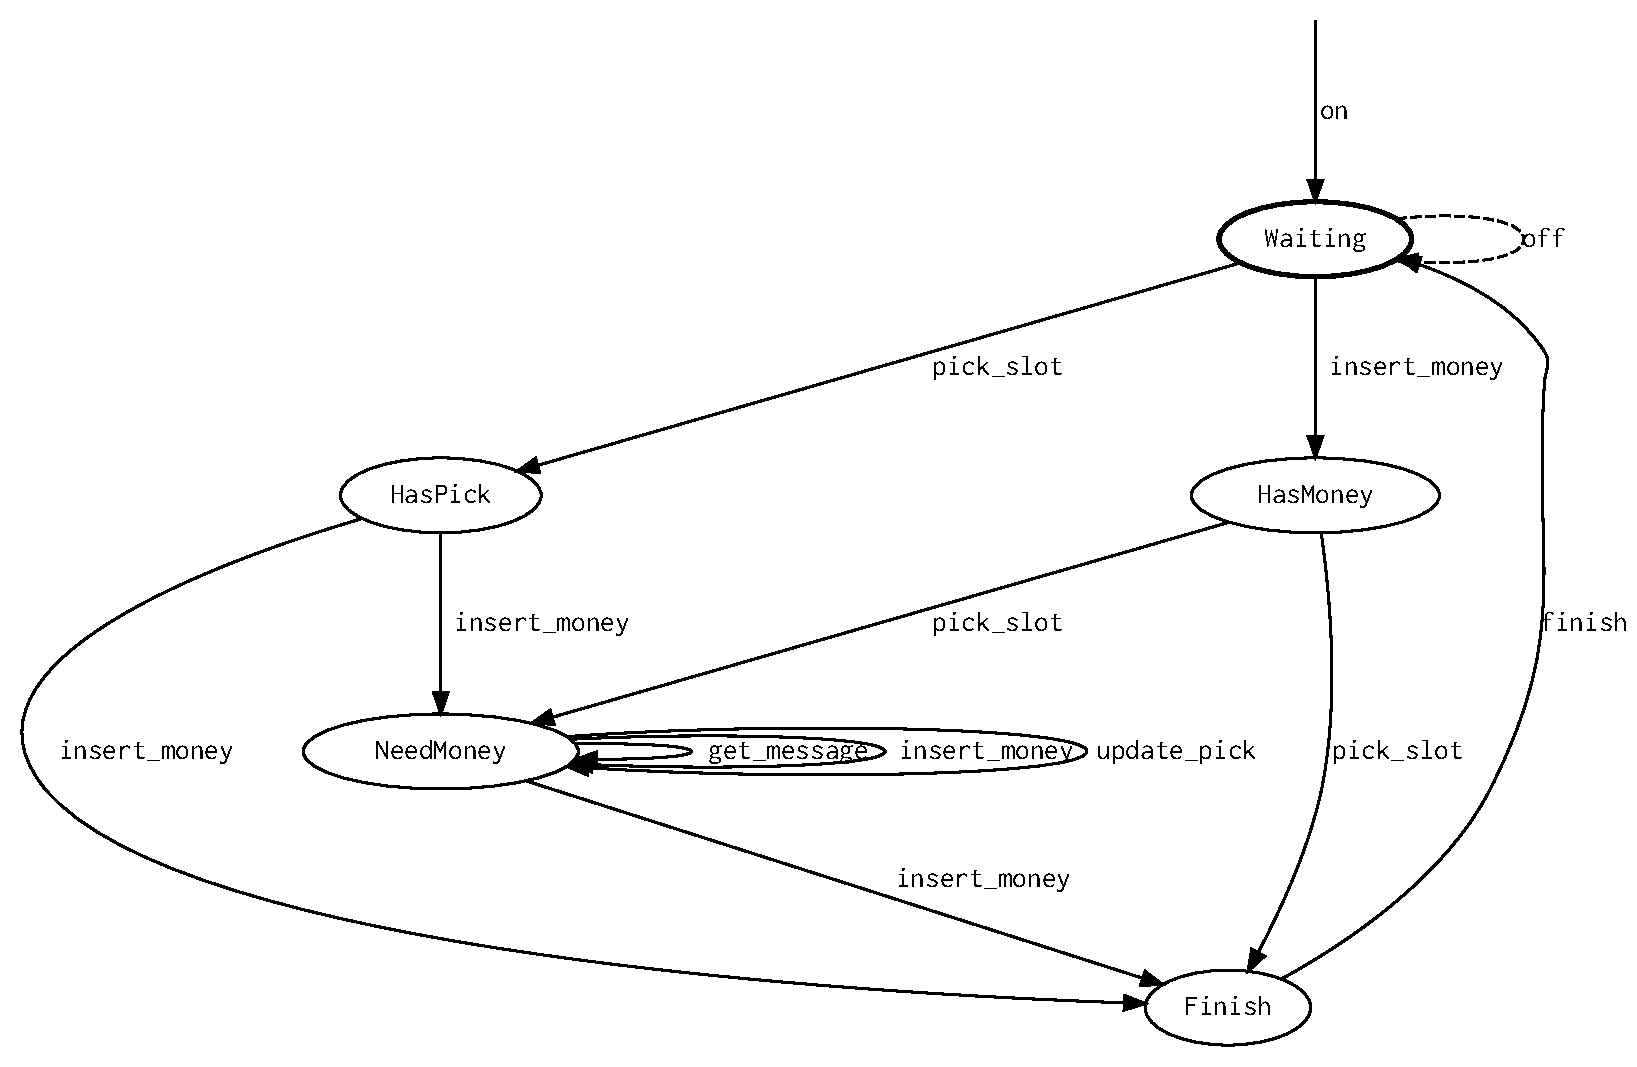
\includegraphics[width=\linewidth]{Chapters/Figures/C4/VendingMachine.dot.pdf}
    \caption{The vending machine's DOT typestate, rendered using the command --- \texttt{dot -Tsvg VendingMachine.dot}.}
    \label{fig:vending-machine-typestate-dot}
\end{figure}

\paragraph{PlantUML} offers the \emph{state diagram} format, providing a more concise way of describing the typestate
by allowing us to have dedicated initial and final states, as well as decision nodes.
Just like the previous feature, exporting PlantUML is done using features;
in this case the flag is \texttt{--features typestate/export-plantuml},
which will export all typestates into separate \texttt{\$TYPESTATE\_NAME.uml} files.


\begin{figure}
    \centering
    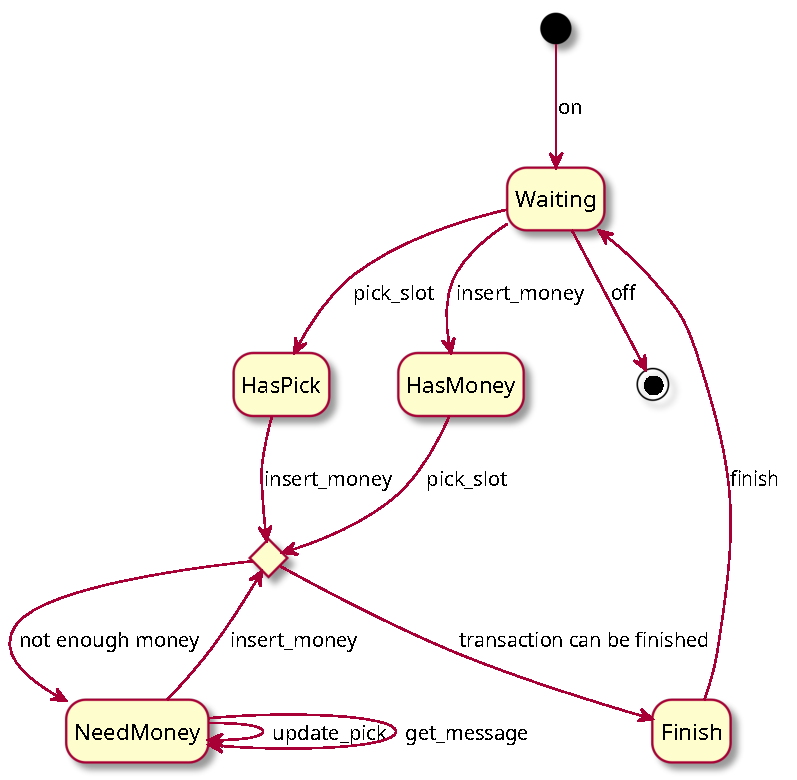
\includegraphics[width=0.7\linewidth]{Chapters/Figures/C4/VendingMachine.uml.pdf}
    \caption{The vending machine's PlantUML typestate, rendered using the command --- \texttt{plantuml -tsvg VendingMachine.uml}.}
    \label{fig:vending-machine-typestate-uml}
\end{figure}

\paragraph{Customization} of the exported formats is possible through environment variables,
these are listed in \autoref{tab:export-env-vars}.

\begin{table}[]
    \centering
    \begin{tabular}{p{0.12\linewidth}|p{0.25\linewidth}|p{0.53\linewidth}}
        Tool                      & Environment Variable       & Description                                                                                                           \\ \hline
        \multirow{3}{*}{DOT}      & \texttt{DOT\_PAD}          & Specifies how much, in inches, to extend the drawing area around the minimal area needed to draw the graph.           \\ \cline{2-3}
                                  & \texttt{DOT\_NODESEP}      & In \texttt{DOT}, \texttt{nodesep} specifies the minimum space between two adjacent nodes in the same rank, in inches. \\ \cline{2-3}
                                  & \texttt{DOT\_RANKSEP}      & In \texttt{DOT}, sets the desired rank separation, in inches.                                                         \\ \hline
        \multirow{2}{*}{PlantUML} & \texttt{PLANTUML\_NODESEP} & \texttt{nodesep} specifies the minimum space between two adjacent nodes in the same rank.                             \\ \cline{2-3}
                                  & \texttt{PLANTUML\_RANKSEP} & Sets the desired rank separation.                                                                                     \\ \hline
        Both                      & \texttt{EXPORT\_FOLDER}    & Declare the target folder for the exported files.
    \end{tabular}
    \caption{All configuration parameters for the DOT and PlantUML visualization features.}
    \label{tab:export-env-vars}
\end{table}

\subsection{Embedding Visualizations in the Documentation}\label{sec:automata-visualization:documentation-generation}

Exporting typestates in a way that enables the developer to visualize them is a valuable tool during development and debugging, also improving communication.
However, when focusing on communication, the best way to ensure the \gls{API} client gets to see the typestate would be to embed it in the documentation;
as documentation is the \emph{de facto} way to communicate between a library's author and its users.

Unfortunately, embedding images in Rust documentation requires a link to that image, which in turn, requires some other place to host the image;
this constraint makes it more complicated to embed the DOT or PlantUML render inside the documentation.
Ideally, we want everything in one place, generated in one step!

Fortunately, \ttt{aquamarine} addresses that problem;
it allows the declaration of Mermaid.js diagrams as documentation and then renders them as HTML inside the Rust documentation.
Its syntax is \emph{very similar} to PlantUML's,
thus this feature's implementation process was mostly porting the PlantUML generation code and fixing any bugs which appeared.

\paragraph{Rendering the state diagram} starts by adding \emph{doc comments}\citeurl{https://doc.rust-lang.org/reference/comments.html\#doc-comments}{20/07/2021}
to the module during the macro processing, the \emph{doc comment} contains the diagram description in the Mermaid.js specification language;
the expanded code for the vending machine example (\autoref{fig:vending-machine}) can be seen in \autoref{lst:vending-machine-mermaid-doc-comment}.
When the user runs the documentation command --- \texttt{cargo doc}; the \ttt{aquamarine} attribute is attached and
the comment is processed by the \texttt{aquamarine} macro, the final diagram is then made available in the documentation;
pictured in \autoref{fig:vending-machine-mermaid-docs}.

\begin{listing}
    \begin{minted}{Rust}
///```mermaid
///stateDiagram-v2
///[*] --> Waiting : on
///state CheckFinish <<choice>>
///CheckFinish --> NeedMoney : not enough money
///CheckFinish --> Finish : transaction can be finished
///HasMoney --> CheckFinish : pick_slot
///HasPick --> CheckFinish : insert_money
///Waiting --> HasMoney : insert_money
///Waiting --> [*] : off
///Waiting --> HasPick : pick_slot
///NeedMoney --> CheckFinish : insert_money
///NeedMoney --> NeedMoney : get_message
///NeedMoney --> NeedMoney : update_pick
///Finish --> Waiting : finish
///```
mod vending_machine_api { /* ... */ }
    \end{minted}
    \caption{\emph{Doc comments} resulting for the expansion of the vending machine example (\autoref{fig:vending-machine}).}
    \label{lst:vending-machine-mermaid-doc-comment}
\end{listing}

\begin{figure}
    \centering
    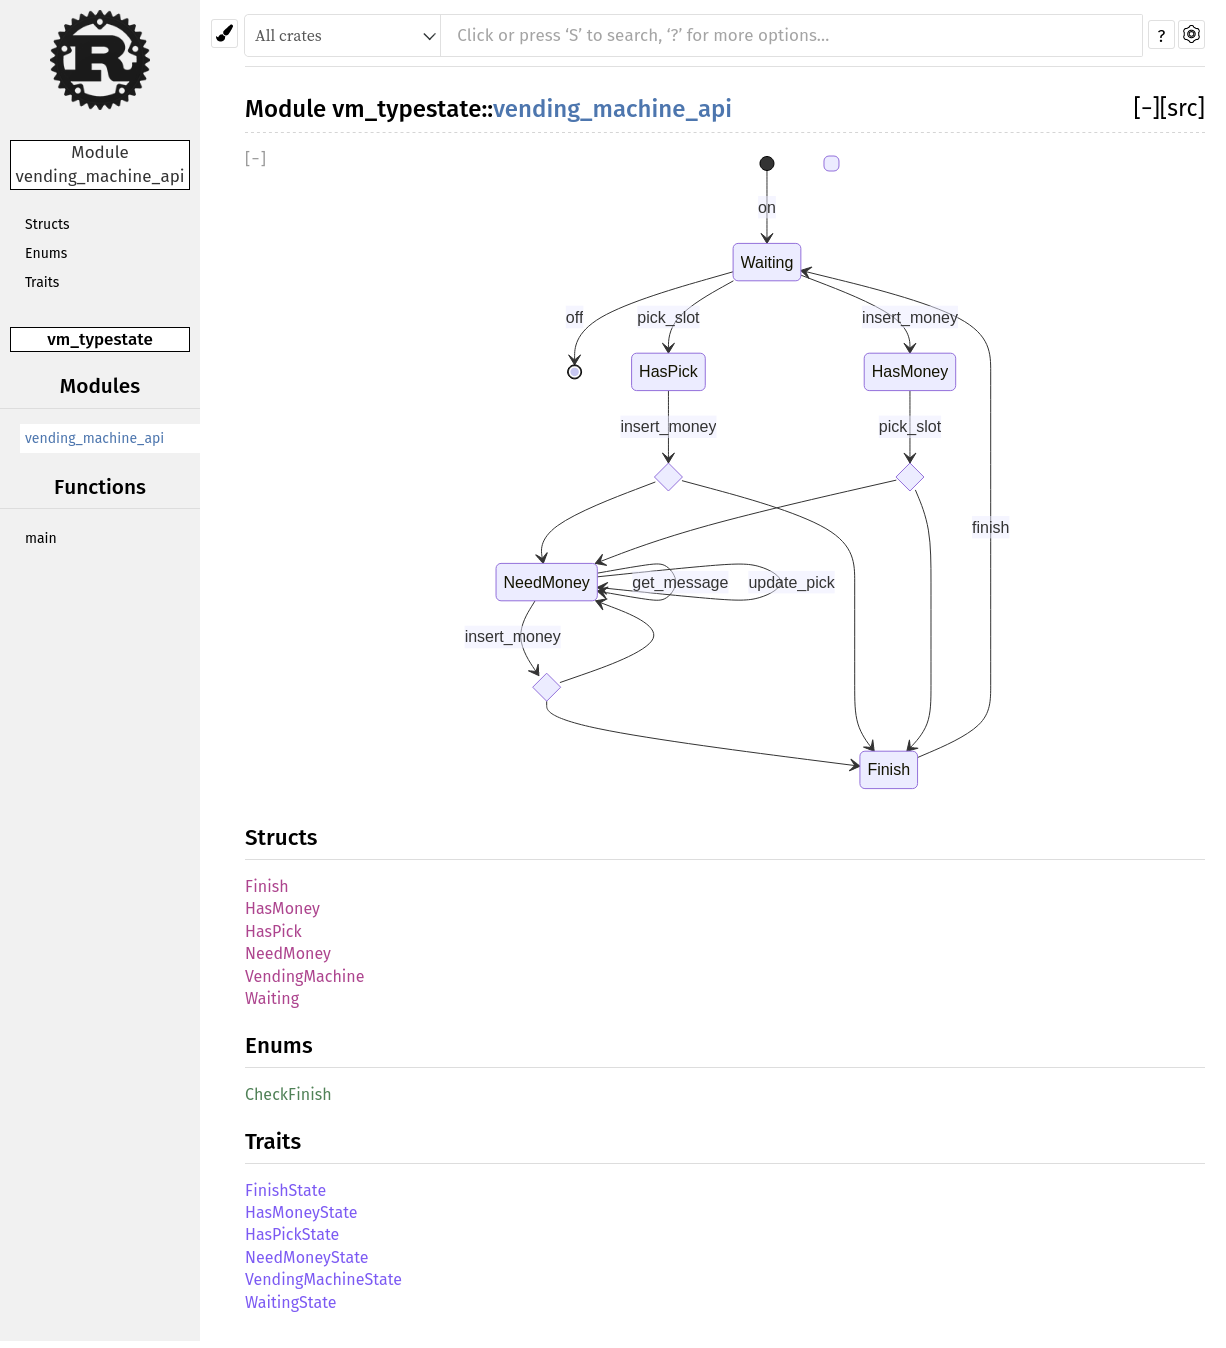
\includegraphics[width=\textwidth]{Chapters/Figures/C4/vending-machine-rustdoc-mermaid.png}
    \caption{
        The vending machine \gls{API} documentation page.
        Result of \autoref{lst:vending-machine-mermaid-doc-comment} when rendered using \texttt{cargo doc}.
    }
    \label{fig:vending-machine-mermaid-docs}
\end{figure}

\paragraph{Bundling the macro} in way that users can depend on this feature is not a trivial task;
we want users to simply import the \texttt{typestate} library and be able to embed their typestates in the documentation.
Rust applies some restrictions to procedural macro libraries, namely,
such libraries cannot export anything else other than the defined macros;
this is a deal-breaker since the \texttt{typestate} crate \emph{is} a procedural macro crate and
forcing the user to explicitly import \ttt{aquamarine} into their project is more overhead than necessary.

The solution for this is to create a \emph{frontend} crate which imports both the \texttt{typestate} macro and \ttt{aquamarine},
and then exports both, this sidesteps the previous issue since the crate exporting the items \emph{is not} the macro crate;
this process is pictured in \autoref{fig:typestate-rs-deps}, \autoref{fig:typestate-rs-deps-naive} and \autoref{fig:typestate-rs-deps-export}.

\begin{figure}
    \centering
    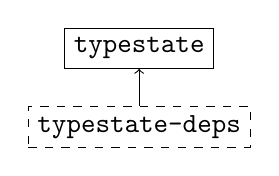
\begin{tikzpicture}
        \node[draw, align=center] (typestate) at (0, 0) {\texttt{typestate}};
        \node[draw, align=center, dashed] (typestate-deps) at (0, -1) {\texttt{typestate-deps}};
        \draw[->] (typestate-deps) -> (typestate);
    \end{tikzpicture}
    \caption[
        The original configuration, the macro depends only on \texttt{typestate-deps} and does not export any dependency.
    ]{ % HACK
        The original configuration, the macro depends only on \texttt{typestate-deps}\footnotemark and does not export any dependency.
    }
    \label{fig:typestate-rs-deps}
\end{figure}

\begin{figure}
    \centering
    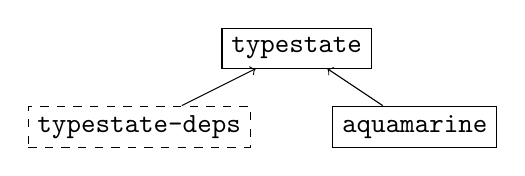
\begin{tikzpicture}
        \node[draw, align=center] (typestate) at (0, 0) {\texttt{typestate}};
        \node[draw, align=center, dashed] (typestate-deps) at (-2, -1) {\texttt{typestate-deps}};
        \node[draw, align=center] (aquamarine) at (1.5, -1) {\texttt{aquamarine}};
        \draw[->] (typestate-deps) -> (typestate);
        \draw[->] (aquamarine) -> (typestate);
    \end{tikzpicture}
    \caption[
        The naive attempt, the macro depends on \texttt{typestate-deps} and \texttt{aquamarine},
        but it only tries to export \texttt{aquamarine}, this fails because \texttt{typestate} is a procedural macro crate.
    ]{ % HACK
        The naive attempt, the macro depends on \texttt{typestate-deps}\footnotemark[\value{footnote}] and \texttt{aquamarine},
        but it only tries to export \texttt{aquamarine}, this fails because \texttt{typestate} is a procedural macro crate.
    }
    \label{fig:typestate-rs-deps-naive}
\end{figure}

\begin{figure}
    \centering
    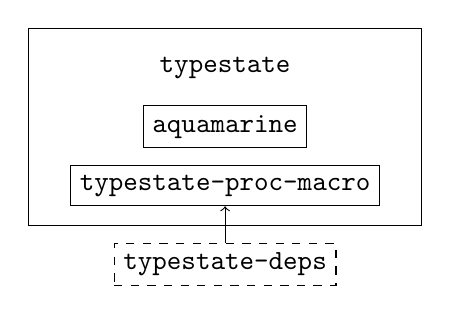
\begin{tikzpicture}
        \draw[] (-2.5, 1) rectangle (2.5, -1.5);
        \node[align=center] (typestate) at (0, 0.5) {\texttt{typestate}};
        \node[draw, align=center] (aquamarine) at (0, -.25) {\texttt{aquamarine}};
        \node[draw, align=center] (typestate-proc-macro) at (0, -1) {\texttt{typestate-proc-macro}};
        \node[draw, align=center, dashed] (typestate-deps) at (0, -2) {\texttt{typestate-deps}};
        \draw[->] (typestate-deps) -> (typestate-proc-macro);
    \end{tikzpicture}
    \caption[
        The macro was isolated in its own crate --- \texttt{typestate-proc-macro}, which depends on \texttt{typestate-deps};
        the \texttt{typestate} crate now depends and exports both \texttt{aquamarine} and \texttt{typestate-proc-macro}.
    ]{ % HACK
        The macro was isolated in its own crate --- \texttt{typestate-proc-macro}, which depends on \texttt{typestate-deps}\footnotemark[\value{footnote}];
        the \texttt{typestate} crate now depends and exports both \texttt{aquamarine} and \texttt{typestate-proc-macro}.
    }
    \label{fig:typestate-rs-deps-export}
\end{figure}

\footnotetext{
    \texttt{typestate-deps} is the set of dependencies for the macro \eg{\texttt{syn}, \texttt{quote}, etc};
    it is dashed as it is not exported.
}

\section{Summary}

In this chapter I have presented:
\begin{compactitem}
    \item How the user can write typestates by hand (\autoref{sec:typestates-hard-way}).
    \item How the DSL is architected, its syntax and more advanced features (\autoref{sec:macro-dsl}).
    \item How the built typestate is validated (\autoref{sec:validation}).
    \item How the user can visualize and document their typestates (\autoref{sec:automata-visualization}).
\end{compactitem}

The use of procedural macros is nothing new to the ecosystem, however, DSLs are usually built with function-like procedural macros.
While such approach has advantages \eg{the usage of new syntax and more expressive constructs} it comes at the cost of not only being harder to develop,
but also requiring the developer to pay the upfront cost of learning it before they can use the DSL.

The present work is by no means final, there is a lot to improve upon (this is detailed in \autoref{cha:conclusions}),
but nonetheless, it achieves interesting insights:


\paragraph{DSLs} do not need to be a complete new language or even extend their host language;
attaching a macro to a module provides a near complete language by itself,
upon which we can simply tweak its semantics to our purposes.

My DSL minimizes the cost of getting up and running by lightly tweaking Rust's semantics and building new constructs on top of it,
such as the automata and state structures.
While learning cost is reduced, a disadvantage is that some users may find the tweaks to be \quotes{non-natural}.

% My DSL tries to minimize these costs by using only existing Rust syntax, only tweaking some semantics.
% This approach has the advantage that learning cost is reduced,
% but the disadvantage that some users may find the semantic tweaking non-natural.

\paragraph{Diagrams} are powerful communication tools, as the popular saying goes --- \equotes{A picture is worth a thousand words}.
Leveraging the graph-like nature of typestates to produce diagrams
provides an extraordinary tool to aid in any development related to the typestate.
Taking advantage of Rust's powerful macro system, one can eventually adapt these to other areas such as session types,
or other areas where the line between code and information is blurred.

To the best of my knowledge, my work is the first to leverage an existing embedded DSL and generate a moderately complex form of documentation.
As a visual-leaning learner, I believe this feature can help users of the final APIs to understand how their typestates work,
especially in more complex settings where state relationships may be difficult to visualize mentally.
Moreover, these diagrams, being specifications, also facilitate debugging, maintenance and extension of the applications.
